%%%%FILE MPL_150_001-043_150_scan031.tex
\scanpage{31}
\mspage{10}
est ``transversal'' i.e. \deleted{\unsure{X|si}} $\exists$ voisinages cylindriques
de $X_{j'}$ \inserted{dans $X_j$} et un de $X_{k'}$ dans $X_k$, tel que l'application
$X_k\unsure{-|\to}X_j$ induit un \deleted{\unsure{hom.}}\inserted{morphisme} sur les
cylindres (compatible avec les structures
cylindriques) et de plus
$\overline E_{\unsure{k';k|k;k}}=p_{jk}^{-1}(\overline E_{\unsure{j';j|j;j}})$.

Système de voisinages cylindriques \deleted{associé}
\inserted{(des $X_{j'}$ dans les $X_j$)}
compatible avec une stratification : tel que
dans b, les \deleted{\unsure{$X$}}$E_{j';j}$ ($j$ fixé, $j'$ prédécesseur)
soient compatibles. Notion correspondante
pour les germes de voisinage cylindrique.

Stratification cylindrique : stratification munie
d'une telle ``structure cylindrique'', en
termes de germes de voisinages cylindriques.

\deleted{\uline{NB} \unsure{Une}}
\uline{NB} Une stratification précylindrique \inserted{resp. cylindrique}
est \unsure{sûrement}
``\unsure{équisingulier|équisingulière}'' au sens le plus fort qu'on
puisse introduire \illegible{1} (\unsure{C|cf.}) suite.

Mais j'ai oublié une condition, que j'exigerai
de tte stratification :
\[
(0)\qquad \forall i,j\in I,\quad\text{on a}\quad
X_i\cap X_j=\bigcup_{k\le i,j}X_k
\]
\margin{\uline{NB} si $i,j$ ont pour borne inf $h$,
cela implique $X_i\cap X_j=X_h$. \unsure{même pour} \illegible{3} \unsure{c)} $\unsure{X_i\cap X_j}$.}

Corollaire : Si $X_i\cap X_j\ne\varnothing$, alors $i,j$ ont un
minorant $\unsure{k|h}$ (tel que \deleted{\unsure{le}} $X_k\ne\varnothing$\ldots)
\margin{30}
%%%%FILE MPL_150_001-043_150_scan032.tex
\scanpage{32}
\mspage{11}
Prenons $T_{I_0}=\coprod_{\beta\in I_0}T_\beta$ voisinage
\deleted{tubulaire}\inserted{cônique} strict
de $X_{I_0}$, supposons le strt transversal aux
$(B_i,\mathcal E_i)$, et \deleted{aux} que les $X_i$
($i\in I^*\overset{\mathrm{def}}=I\setminus I_0$)
soient str. admissibles pour $\overline T_{I_0}$.

Notons que en vertu de (14), si $\beta\in I_0$ donc
minimal dans $I$, donc pour $i\in I$ on a
\[
(14)\qquad
X_i\cap X_\beta=
\begin{cases}
\varnothing & \text{si }\deleted{\beta}i\not\ge\beta\\
X_\beta & \text{sinon \unsure{i.e.} }i\ge\beta\quad(\text{ceci est trivial})
\end{cases}
\]
Soit $I_\beta$\inserted{$\subset I^*$} l'ens des $i\in I$ tels que $i>\beta$.
On a donc
\[
(15)\qquad i\in I^*\setminus I_\beta\quad\Longrightarrow\quad
X_i\cap\overline T_\beta=\varnothing
\]
(car $X_i\cap X_\beta=\varnothing$ et $X_i$ admissible pour $\overline T_\beta$),
\[
(16)\qquad i\in I_\beta\quad\Longrightarrow\quad X_i\supset X_\beta
\]
Donc on a
\[
(16')\qquad X_i\cap T_\beta
=I.\underbrace{X_i\cap\dot T_\beta}_{\dot X_i}\cup X_\beta
\]

Ainsi, le système
\[
(17)\qquad
(X,(X_i)_{i\in I},(B_\alpha,\mathcal E_\alpha)_{\alpha\in R}
(\mathcal T_\beta)_{\beta\in I_0})
\]
se reconstitue à l'aide de
\inserted{$(X_\beta)_{\beta\in I_0},$}

\deleted{
\[
(18)\quad
\left(
\underset{\substack{\parallel\\X\setminus\mathring T_{I_0}}}{X^*},
\left(\underset{\substack{\parallel\\\dot T_\beta}}{\dot X_\beta}\right)_{\beta\in I_0},
\left(\underset{\substack{\parallel\\B_\alpha\cap X^*}}{B_\alpha^*},
\underset{\substack{\parallel\\\mathcal E_\alpha\cap X^*}}{\mathcal E_\alpha^*}\right),
\left(\underbrace{(X_{\beta\alpha},\mathcal E_{\beta\alpha})}
_{=(B_{\unsure{\alpha}}^*,\mathcal E_\alpha^*)|X_\beta}\right)_{\beta\in I_0}
\right)
\]
\[
(\dot X_\beta\longrightarrow X_\beta)_{\beta\in I_0}
\]
}
\margin{31}
%%%%FILE MPL_150_001-043_150_scan033.tex
\scanpage{33}
\mspage{12}
\[
(18)\quad\left\{
\begin{gathered}
\underset{\substack{\parallel\\X\setminus\mathring T_{I_0}}}{X^*},
\overbrace{
\left(\underset{\substack{\parallel\\\dot T_\beta}}{\dot X_\beta},
\unsure{\mathcal E_\beta}\right)_{\beta\in I_0},
\underbrace{(B_\alpha^*,\mathcal E_\alpha^*)}
_{(B_\alpha,\mathcal E_\alpha)|X^*}{}_{\alpha\in\Lambda}
}^{\substack{\text{syst. de cylindres-bord}\\\text{transversaux}}},
\left(\underset{\substack{\parallel\\X_i\cap X^*}}{X_i^*}\right)_{i\in I^*};
(X_\beta)_{\beta\in I},
\underbrace{(B_{\beta,\alpha},\mathcal E_{\beta,\alpha})}
_{(B_\alpha,\mathcal E_\alpha)|X_\beta}
{}_{\substack{\alpha\in\Lambda\\\beta\in I_0}},\\
(\dot X_\beta\overset{p_\beta}\longrightarrow X_\beta)_{\beta\in I_0}
\end{gathered}\right\},
\]
de la façon suivante :

\margin{les $\dot X_\beta$ disjoints}
\[
(19)\quad\left\{
\begin{aligned}
\widehat X&=X^*\amalg_{\dot X=\coprod\dot X_\beta}
\underbrace{C(p=\coprod p_\beta)}
_{\deleted{\unsure{I}}\coprod_\beta C(p_\beta)},\\
T_\beta&=C(p_\beta)\\
X_\beta&\quad\text{pour }\beta\in I_0\quad\text{clair}.\\
X_i&\quad\text{pour }i\in I^*\text{ est donné par }
\deleted{\unsure{X_i=I.\dot X_i}}\\
\deleted{\unsure{X_i}}\quad X_i&=X_i^*\deleted{\unsure{\cup}}
\cup\bigcup_{\substack{\beta\in I_0\\\beta\le i\\\deleted{\unsure{i\in I_\beta}}}}
\left(I.\underbrace{\dot X_{i\beta}}
_{\substack{\parallel\mathrm{def}\\X_i^*\cap\dot X_\beta}}
\deleted{\unsure{I.(X_i^*\cap\dot X_\beta)}}\cup X_\beta\right)\\
B_\alpha&=B_\alpha^*\cup\bigcup_{\beta\in I_0}
I\underbrace{\dot B_\alpha}_{\substack{\parallel\mathrm{def}\\B_\alpha^*\cap\dot X_\beta}}\\
\mathcal E_\alpha&\quad\text{défini par }\mathcal E_\alpha^*
\text{ et les }(B_{\beta,\alpha},\mathcal E_{\beta,\alpha})
\end{aligned}\right.
\]

\uline{Conditions} sur (18)
\[
(20)\quad\left\{
\begin{array}{l}
\text{\textcircled{a} Les }X_\beta\text{ disjoints}\\
\text{\textcircled{b} Chaque }\dot X_\beta\text{ transverse à }(B_\alpha^*,\mathcal E_\alpha^*)
\end{array}\right.
\]
\margin{$\Longrightarrow$ le syst. des $(\dot X_\beta,\unsure{\mathcal E_\beta})$,
$(B_\alpha^*,\mathcal E_\alpha^*)$ est \unsure{transverse}}

\textcircled{d}
\[
(\dot X_\beta,
\underbrace{\dot B_{\beta\alpha},\dot{\mathcal E}_{\beta\alpha}}
_{\substack{\text{induit sur }\dot X_\beta\\
\text{par }(B_\alpha^*,\mathcal E_\alpha^*)}})
\longrightarrow
(X_\beta,B_{\beta,\alpha},\dot{\mathcal E}_{\beta,\alpha})
\]
est transverse

\inserted{\textcircled{\unsure{c}} Les $X_i^*$ transverses aux
$\big((\dot X_\beta,\mathcal E_\beta)_{\beta\in I_0},
(B_\alpha^*,\mathcal E_\alpha^*)_{\alpha\in\Lambda}\big)$}
\margin{32}
%%%%FILE MPL_150_001-043_150_scan034.tex
\scanpage{34}
Il faut de plus des conditions qui assurent,
à partir des données (18), que $i\mapsto X_i$
est croissant, et \deleted{que} la condition (14)
$X_i\cap X_j=\bigcup_{k\le i,j}X_k$. Pour \deleted{les} exprimer ces conditions,
on introduit pour tt $\beta\in I_0$ l'ens
\[
(21)\qquad I_\beta^*=\{i\in I^*\mid i>\beta\}
\]
donc la donnée de $(I\supset I')$
\inserted{($I$ ens. ordonné)} équivaut à celle
de $I^*,I_0$ \inserted{(ens. ordonné \quad ens.)} et de la famille des
$I_\beta^*\subset I^*$ ($\beta\in I_0$).

Pour \deleted{vérifier}\inserted{exprimer} que \deleted{$X_i$}
$i\le j$ \inserted{(donc $j\in I^*$)} implique $X_i\subset X_j$,
on distingue les cas où $\underset{\substack{\Vert\\\beta}}{i}\in I_0$
\deleted{\unsure{ou}}, où c'est
clair sur (19), et celui où $i\in I^*$ où \deleted{et} c'est
clair aussi sur (19), compte tenu de la condition
néc. évidente
\[
\text{e)}\qquad \deleted{\unsure{\forall}} i,j\in I^*,\ i\le j
\quad\Longrightarrow\quad X_i^*\subset X_j^*
\]
\deleted{Pour que}\inserted{On doit} avoir aussi, manifestement
\[
\text{f)}\qquad \unsure{j|i},j\in I^*\Longrightarrow
X_i^*\cap X_j^*=\bigcup_{k\le i,j}X_k^*
\]

Pour la relation
\[
X_i\cap X_j=\bigcup_{k\le i,j}X_k\qquad(i,j\in I)
\]
il \deleted{de} suffit de prendre le cas où $i,j$ ne
sont pas comparables. Quand un des deux
est $\in I_0$, alors cette relation \deleted{est} signifie que
$\beta\in I_0$, $i\in I^*\setminus I_\beta$, on a
$X_\beta\cap X_j=\varnothing$, ce qui résulte de (19).
\margin{33}
%%%%FILE MPL_150_001-043_150_scan035.tex
\scanpage{35}
\mspage{13}
Si $i,j\in I^*$, il suffit \inserted{(grâce à f))}
de vérifier que pour tt
$\beta$, on a
\[
X_i\cap X_j\cap T_\beta=\bigcup_{k\le i,j}X_k\cap T_\beta
\]
(il suffit de prouver $\subset$, car $\supset$ trivial). Si
$X_i\cap X_j\cap T_\beta=\varnothing$ c'est trivial, on peut donc supposer
$X_i\cap X_j\cap T_\beta\ne\varnothing$
\deleted{\unsure{i.e.} $X_i\cap X_j\cap$}
donc $X_i\cap T_\beta\ne\varnothing$, $X_j\cap T_\beta\ne\varnothing$
i.e. $i,j\in I_\beta$. Alors \deleted{\unsure{de}} cela résulte de
(f) induit sur $\dot T_\beta=\dot X_\beta\subset X^*$,
et de la formule (19). Donc

\uline{Thm} Les systèmes (17), satisfaisant aux
conditions \deleted{\unsure{tt}} (14) des stratifications, et aux
conditions de transversalité explicitées plus
haut, équivalent aux systèmes (18), satisfaisant
aux conditions (20), en plus des conditions
e) f) exprimant que les $(X_i^*)_{i\in I^*}$ forment une
stratification de $X^*$.

8. \uline{Structure cônique sur un espace stratifié}

Pour $X$ stratifié de type $I$ par des
$(X_i)_{i\in I}$, avec des sous-espaces bordants donnés
\inserted{$(B_\alpha)_{\alpha\in\Lambda}$}
et des germes de \inserted{voisinages} cylindriques des $B_\alpha$, tel que
\deleted{\unsure{ces bords} \unsure{de} \unsure{manière}}
les $(B_\alpha)$ soient mutuellement transverses, et
transverses aux $X_i$, on va \deleted{construire} définir
\margin{34}
%%%%FILE MPL_150_001-043_150_scan036.tex
\scanpage{36}
par récurrence sur $\operatorname{card}I$ la notion de
\unsure{donnée|données} \deleted{de} côniques sur \deleted{cette base}
$(X,(X_i)_{i\in I},(B_\alpha,\mathcal E_\alpha)_{\alpha\in\Lambda})$.
\deleted{On procède} Si $I=\varnothing$, ce sera la structure
vide (il y en a une et une seule). Si
$I\ne\varnothing$, on prend $I_0$ ens des éléments minimaux
de $I$, et une donnée cônique sera par
définition la donnée

\textcircled{a} d'un \deleted{tube}\inserted{vois. con. strict} $\overline T_{I_0}$
de \deleted{\unsure{la somme}} $X_{I_0}=\bigcup_{\beta\in I_0}X_\beta$,
transversal aux $(B_\alpha,\mathcal E_\alpha)$ et
\deleted{\unsure{donc} admissible}
côniquement transversal aux $X_i$ ($i\in I$).
--- ce qui permet donc d'introduire les
structures (19), et en particulier

\[
(22)\qquad
X^*,\quad
\underbrace{(X_i^*)_{i\in I^*=I\setminus I_0}}
_{\text{stratification de }I^*},
\quad
\underbrace{\big((\deleted{\mathcal E}B_\alpha,\mathcal E_\alpha)_{\alpha\in\Lambda},
(\dot X_\beta,\mathcal E_\beta)_{\beta\in I_0}\big)}
_{\substack{\text{famille transverse}\\\text{de sous-espaces}\\
\text{bordants ``cylindrisés''}\\
\text{de }X,\ \text{transversaux}\\\text{aux }X_i}}
\]

en plus de
\[
(23)\qquad
\big((X_\beta)_{\beta\in I_0},
(B_{\beta\alpha},\mathcal E_{\beta\alpha})_{\substack{\beta\in I_0\\\alpha\in\Lambda}}\big)
\]
On doit avoir de plus : $\unsure{\infty|a}$

\textcircled{b} Une structure cônique sur (22) (ce qui
a un sens, par récurrence\ldots)
\margin{35}
%%%%FILE MPL_150_001-043_150_scan037.tex
\scanpage{37}
\mspage{14}

\deleted{\unsure{NB}}\quad \uline{Remarques}\quad
1) Avec des hypothèses de ``non sauvagerie'' sur la donnée initiale
\[
 (X,(X_i)_{i\in I},(B_\alpha,\mathcal E_\alpha)_{\alpha\in\Lambda}),
\]
il doit être vrai qu'il existe une structure cônique. Si la stratification
\deleted{\unsure{X}} est équisingulière le long de tout
\[
 X_i^\circ\mathrel{\mathop=^{\mathrm{déf}}}
 X_i\setminus\bigcup_{\substack{j<i\\\unsure{j\le i}}}X_j,
\]
alors il doit \(\unsure{=}\) y avoir une structure cônique équisingulière
(avec la définition ad-hoc évidente) --- il suffit de savoir construire
un tube équisingulier autour des \(X_{I_0}\) \(\cdots\)

2) A priori, si on a une suite \inserted{str.} croissante
de parties
\[
 \varnothing\subset I_0\subset I_1\cdots\subset I_{\unsure{n-1}}\subset I_{\unsure{n|N}}=I,
\]
avec \deleted{\(I_i\) formé d'él. minim.}
\inserted{\(\forall i\)} \(I_i\setminus I_{i-1}\) formé d'él. minimaux
de \(I\setminus I_{i-1}\), alors on pourrait définir
\inserted{par récurrence} une notion de structure cônique
pour cette ``filtration'' de \(I\). Mais on
peut montrer que cette notion ne dépend pas
en fait, essentiellement, de la filtration
choisie.

3) Au lieu d'une famille des \((B_\alpha,\mathcal E_\alpha)_{\alpha\in\Lambda}\),
on peut supposer donnée sur \(X\) une
stratification cylindrique \deleted{de type} (le cas envisagé
est celui où l'ens ordonné qui \deleted{\unsure{poin\ldots|porte}}
\unsure{décrit|indexe} la stratification cylindrique est
\(\mathcal P(\Lambda)^\circ\).

\margin{36}
%%%%FILE MPL_150_001-043_150_scan038.tex
\scanpage{38}
Il n'y a pas de différence essentielle avec
le traitement fait ici. Plus tard on
généralisera cette notion de stratification
cylindrique (globale) en une notion de
stratification cylindrique locale --- et ce sera
la même \unsure{théorie}.

9. \uline{Description d'une} \deleted{structure}
\inserted{stratification} \uline{cônique} \uline{de type} \(I\)
(\(I\) un ordonné fini).

Pour simplifier, on prend \inserted{d'abord} le cas où on
ne se donne pas de \unsure{stratifications cylindriques|stratification cylindrique}
sur \(X\) \unsure{par dessus le marché|pour donner des ennuis}.

\deleted{\unsure{Soit}}

\margin{37}
%%%%FILE MPL_150_001-043_150_scan039.tex
\scanpage{39}
\mspage{15}

Stratification \deleted{\unsure{équisingulière}}\inserted{équisingulière}
de type \(I\) (\(I\) ens. ordonné fini) : présentation standart.
On suppose donnée une ``catégorie topologique modérée'' \(\mathcal M\)
(\deleted{\illegible{1}} \unsure{en} un sens non précisé, pour que ça puisse être aussi celle des
espaces topologiques \(\cdots\)). La présentation est donnée
par un \inserted{contr.} foncteur
\[
 \begin{aligned}
 \Sigma:\ \operatorname{Drap}(I)&\longrightarrow\mathcal M\\
 (i_0,\ldots,i_n)&\longmapsto\Sigma_{i_0\ldots i_n}
 \end{aligned}
\]
avec les propriétés suivantes

(1) Le \deleted{\unsure{app}} morphisme
\[
 \Sigma_{i_0\ldots i_n}\longrightarrow\Sigma_{i_0,\ldots,i_p}
\]
(relatif à une inclusion de drapeaux
\(d\unsure{\hookrightarrow}d'\) telle
que \(d\) soit un segment initial de \(d'\)\inserted{\(\unsure{p}\)\quad\(\unsure{n}\)}) est \uline{fibrant}\(^*\).

\margin{NB \inserted{on} \unsure{ne poser}
cette condition que dans le cas équisingulier.}

\margin{\(^*\) Cela est trop faible, \unsure{si on veut|$=$ pour}
l'équisingularité --- il faut
supposer que pour \(d\) fixé, et pour
\(d'\unsure{\supset|=}d\amalg\delta\) \unsure{variable}
(où \(\delta\) est \unsure{donc}
un drapeau quelconque de
l'ens \(I'\) des \(i\in I\) \unsure{fort\(^{t}\)|fortement} \uline{\unsure{supérieur|supérieurs}}
\unsure{à} \(\unsure{\max} i_p\))
la \deleted{\unsure{famille}}\unsure{stratification}
qu'ils forment au dessus de
\(\Sigma_{d'}\) est loc. triviale.}

\deleted{(2)} (\deleted{\unsure{Enfin}} il suffit de le supposer pour
\[
 \Sigma_{i_0\ldots i_n}\longrightarrow\Sigma_{i_0\ldots i_{n-1}}
\]
)

(2) Le morphisme
\[
 \deleted{\unsure{\Sigma_{d'}}\longrightarrow\Sigma_d}
 \qquad
 \Sigma_{i_0\ldots i_n}
 \longrightarrow
 \Sigma_{i_0\ldots\widehat{i_p}\ldots i_n},
 \qquad \boxed{p\ne n}
\]
est un plongement-bord
\inserted{i.e. plongement \inserted{\unsure{bord}} cylindrique}
(NB si \(p=n\), c'est un morphisme fibrant.)

\margin{On va supposer
de plus \unsure{données|donnés}
une \deleted{\unsure{famille}} \inserted{des}
structures cylindriques
correspondantes, et \unsure{formuler}
des conditions plus fortes que
(2), \unsure{énoncées en langage}
\unsure{suivant} ---}

\uline{Cor.} Soit \(d\unsure{\hookrightarrow}d'\)
tel que \(d\) et \(d'\) aient \(\unsure{=}\)
\unsure{objt maximals}, alors
\(\Sigma_{d'}\longrightarrow\Sigma_d\) est un plongement.

\deleted{\unsure{(3)}}

\margin{38}
%%%%FILE MPL_150_001-043_150_scan040.tex
\scanpage{40}
\margin{\(^*\) Il suffit \unsure{pour que l'on ait} que
\(\delta=d\cap d'\) soit segment initial de \(d'\) et contienne
le plus grand élément de \(d\), ce qui \unsure{signifie par|dit que pour les}
\(\textcircled{D}\), \(\Sigma_d-\Sigma_\delta\) est
\unsure{mono.} et \(\Sigma_{\unsure{d''|d'}}-\Sigma_d\) est fibrant.}

(3) Soient \(d,d'\) deux drapeaux tels que \inserted{\unsure{sans plus}\(^*\)}
le dernier élément \inserted{\(i\)} de \(d\) soit le premier élément de \(d'\)
et considérons \(d''=d\cup d'\) et le diagramme
\diagram{\begin{tikzcd}
 \Sigma_{d''}\arrow[r,hook]\arrow[d]&\Sigma_{d'}\arrow[d]\\
 \Sigma_d\arrow[r,hook]&\Sigma_i
\end{tikzcd}}
\unsure{ce dernier|est}
est \uline{cartésien}. (Pour \(d\) ou \(d'\)
de longueur \(0\) i.e. réduit à \(\{i\}\), cette condition
est triviale.)

\margin{Il suffit de le supposer pour
\(d\) de longueur \(2\) (ou \(d'\) de longueur \(2\)).
On en déduit plus
\deleted{\unsure{la généralité que si}}
\deleted{\unsure{quelconques}}
\(d,d'\) sont deux drapeaux tels que
\inserted{\(d''=d\cup d'\)}
soit un drapeau et que
\(\delta=d\cap d'\)
\deleted{\(d\cup d'\)}
\(d''=d\amalg_\delta d'\)
\unsure{cat. ou un} \deleted{\unsure{ens}} ordonné,
\(^*\) alors
\[
 \textcircled{D}
\]
\diagram{\begin{tikzcd}
 \Sigma_{d''}\arrow[r]\arrow[d]&\Sigma_{d'}\arrow[d]\\
 \Sigma_d\arrow[r]&\Sigma_\delta
\end{tikzcd}}
est cartésien.}

\margin{De plus, il faut supposer que lorsque
\(d\) est de longueur \(2\), alors
\([\Sigma_{d'}\unsure{-|\longrightarrow}\Sigma_\delta]\) est
\uline{transverse} aux sous-espaces cylindriques \(\Sigma_d\) de
\(\Sigma_{\unsure{\delta}}\) --- et idem pour les structures cylindriques.}

\margin{(\unsure{comme au n° précédent})
On suppose de
plus que \deleted{\unsure{d'ailleurs}} si pour \(i\in I\),
\(\operatorname{Dr}(I,i)\) désigne le sous-ens ordonné
de \(\operatorname{Dr}(I)\) formé des drapeaux
\(d\) dont le dernier élément est \(i\),
de sorte que les \(\Sigma_d\) sont \(\subset\Sigma_i\),
alors les \(\Sigma_d\) forment dans \(\Sigma_i\) une
\uline{stratification précylindrique} de
type \(\operatorname{Dr}(I,i)^\circ\), ce qui s'exprime par
les conditions supplémentaires
\[
 \text{a)}\quad \Sigma_{kj}\cap\Sigma_{\ell j}=\varnothing
 \quad\text{si }k,\ell\unsure{\le}j\text{ sont des noncomparables}.
\]
\[
 \text{b)}\quad
 \Sigma_{i_0\ldots i_n}
 =\Sigma_{i_0i_n}\cap\Sigma_{i_1i_n}\cdots
 \cap\Sigma_{i_{n-1}i_n}
 \qquad\text{dans }\Sigma_{i_n}
\]
\[
 \left(\Longleftrightarrow\
 \Sigma_d\cap\Sigma_{d'}=
 \begin{cases}
 \varnothing&\text{si }d\cup d'\text{ \unsure{pas un drapeau}}\\
 \Sigma_{d\cup d'}&\text{sinon}
 \end{cases}\right)
\]
c) L'intersection dans b) est transversale.
On suppose plus précisément, \unsure{choisis|choisies} des structures
cylindriques \unsure{qui rendent transversales}
\(\Sigma_{ij}\) \(\unsure{(i<j)}\).}

Cela nous donne un procédé \unsure{canonique} pour
reconstruire les \(\Sigma_d\), à isom. \inserted{can.} près,
quand on connaît les \(\Sigma_i,\Sigma_{ij}\)
\inserted{\((i<j)\)} et les morphismes
\diagram{\begin{tikzcd}
 \Sigma_{ij}\arrow[r,hook]\arrow[d]&\Sigma_j\\
 \Sigma_i&
\end{tikzcd}}
\deleted{Pour}
(NB \unsure{que}
la flèche verticale est fibrante, et l'horizontale
un morphisme-bord). Pour avoir les
morphismes de transition entre les
\(\Sigma_d\) (construits par récurrence sur \(\operatorname{long}d\),
les \(0\) et \(1\) étant déjà donné) il faut se donner
les morphismes
\[
 \underbrace{\Sigma_{ij}\mathbin{\times_{\Sigma_j}}\Sigma_{jk}}
 _{\mathrel{\mathop=^{\mathrm{déf}}}\Sigma_{ijk}}
 \longrightarrow\Sigma_{i,k}
\]
satisfaisant aux conditions

\margin{39}
%%%%FILE MPL_150_001-043_150_scan041.tex
\scanpage{41}
\mspage{16}

La donnée des \(\Sigma_i\) équivaut à la donnée d'un
\[
 \Sigma_*\in\mathcal M\qquad
 \left(\Sigma_*=\coprod\Sigma_i\right)
\]
et d'une partition de type \(I\) de \(\Sigma_*\) i.e. d'un morphisme
\[
 \Sigma_*\longrightarrow I_{\mathcal M}.
\]
Celle des \(\Sigma_{ij}\) équivaut à celle
d'un objet \(\Sigma_{**}\) \deleted{\unsure{et|de}} \unsure{au} dessus de \(I\times I\)
\deleted{\(\operatorname{Drap}_{\unsure{1|2}}(I)\)}
\deleted{\(\unsure{I\times I}\)}
(on pose \(\Sigma_{ij}=\varnothing\) si \(i\not\le j\),
\(\Sigma_{ii}=\Sigma_i\)).

La donnée des
\diagram{\begin{tikzcd}
 \Sigma_{ij}\arrow[r,hook]\arrow[d]&\Sigma_j\\
 \Sigma_i&
\end{tikzcd}}
équivaut à celle de deux morphismes ``source'' et ``but''
\diagram{\begin{tikzcd}
 \Sigma_{**}\arrow[r,"\underline b"]\arrow[d,"\underline s"']&\Sigma_*\\
 \Sigma_*&
\end{tikzcd}}
compatibles avec les \(\operatorname{pr}_1\) et \(\operatorname{pr}_2\)
de \(I\times I\) dans \(I\)
(\deleted{\uline{NB} \unsure{le cas}}
\unsure{car|Comme} la bigraduation \inserted{de type \(I\)}
de \(\Sigma_{**}\) est déduite de \deleted{\unsure{celle}}
\unsure{graduation} de type \(I\) de \(\Sigma_*\), et des
\(\underline b\) et \(\underline s\)) ---
\unsure{où} \(\underline b\) est \inserted{\unsure{loc.\(^{t}\)}}
un morphisme bord (i.e. est une
immersion \deleted{\unsure{bord}}) et \(\underline s\) est une fibration.

On a de plus \unsure{a}
\[
 \underline{i}:\ \Sigma_*\unsure{-|\longrightarrow}\Sigma_{**}
\]
``morphisme identité'', dont le composé avec \(\underline b\) et
\(\underline s\) est l'identité. La donnée des
\(\Sigma_{ijk}\unsure{-|\longrightarrow}\Sigma_{ik}\) revient à

\margin{40}
%%%%FILE MPL_150_001-043_150_scan042.tex
\scanpage{42}
une \uline{application} \uline{composition}, et l'axiome à
formuler pour avoir une extension \deleted{en}
\inserted{des \(\Sigma_i,\Sigma_{ij}\)}
en des \(\Sigma_{i_0\ldots i_n}\), est que cette composition
(qui est compatible avec les unités, \unsure{manifestement},
par construction) soit une structure de
\uline{\(\mathcal M\)-catégorie}\(^*\). \deleted{\unsure{une}}
Donc la donnée de \(\Sigma\) satisfaisant (3)
équivaut à celle \unsure{d'une|d'un} \unsure{Catégorie dans|Cat-objet de} \(\mathcal M\),
au dessus de la catégorie \(I_{\mathcal M}\) :
\[
 \Sigma_{\mathcal M}\longrightarrow I_{\mathcal M}.
\]

\margin{\(^*\) En fait, c'est un objet
\uline{ordonné} de \(\mathcal M\), et
\(\Sigma_{i_0\ldots i_n}\) s'identifie à l'ens des drapeaux
\[
 x_{i_0}\le x_{i_1}\le\cdots\le x_{i_n}
\]
de \(\Sigma_*\), au dessus des drapeaux
\(i_0-\cdots-i_n\) de \(I\).
Donc pour vérifier \unsure{(cf. p. 15', marge)}
\[
 \Sigma_{i_0\ldots i_n}
 =\Sigma_{\unsure{i_0i_1|i_0i_n}}\cap\cdots
 \cap\Sigma_{\unsure{i_0i_n}}
\]
il suffit de le vérifier pour \(n=2\), i.e.
\[
 \Sigma_{\unsure{ijk}}=\Sigma_{ik}\cap\Sigma_{jk},
\]
ce qui signifie que pour
tt \(z\in\Sigma_k\), \(\Sigma_*\unsure{-|\longrightarrow}I\) induit
\diagram{\begin{tikzcd}[column sep=large]
 \Sigma_*(z)\arrow[r,hook]\arrow[d,equal]&I(k)\arrow[d,equal]\\
 \{x\in\Sigma_*\mid x\le z\}&\{i\in I\mid i\le k\}
\end{tikzcd}}
qui est tel que l'ordre de \(\Sigma(z)\)
soit \uline{induit} par celui de \(I(k)\).
\deleted{Cela signifie}}

A l'aide de ces données, je vais
construire un espace stratifié de type \(I\),
sans utiliser en fait \deleted{aucune des hypothèses}
\inserted{les \deleted{\unsure{deux}} conditions}
(1) \deleted{et (2)}, la condition (2) n'intervenant
que sous la forme plus faible que
\[
 \Sigma_{i_0\ldots i_n}
 -\Sigma_{i_0\ldots\widehat{i_p}\ldots i_n}\qquad(p\ne n)
\]
est un plongement \deleted{\unsure{bord}}
(\unsure{si on ne veut pas construire} les structures côniques
relatives à l'espace stratifié obtenu).

Je considère pour ceci les couples
\deleted{\(d,d'\)} \((d\subset d')\) de deux drapeaux,
\deleted{\unsure{une}} tels que
\(d\) \deleted{de \(d'\)} ne soit pas cofinal dans \(d'\).
(Pour \(d'\) \inserted{\(=\{i_0,\ldots,i_n\}\)}
\deleted{de longueur \(n\)}
il y a donc \(2^n\) choix possibles pour \(d\)).

\margin{41}
%%%%FILE MPL_150_001-043_150_scan043.tex
\scanpage{43}
\mspage{17}

On considère que cette donnée équivaut à celle d'une
suite d'inclusions de drapeaux
\[
 d_1\subset d_2\cdots\subset d_p\subset d_{p+1}=d'
 \qquad(p=\operatorname{long}.d')
\]
dont chacun est un segment initial strict \unsure{dans|de}
le \deleted{\unsure{précédent}}\inserted{suivant}.
Ceci donne donc \deleted{des filt} une
suite de projections
\[
 \Sigma_{d'}=\Sigma_{d_{\unsure{p+1|p-1}}}\unsure{-|\longrightarrow}\Sigma_{d_p}
 \unsure{-|\longrightarrow}\cdots\unsure{-|\longrightarrow}\Sigma_{d_2}
 \unsure{-|\longrightarrow}\Sigma_{d_1}
\]
dont on considère le mapping-cône simultané
qu'on désigne par
\[
 C_\Sigma(d_1,d_2,\ldots,
 \underset{\substack{\Vert\\d'}}{d_{\unsure{p+1|p-1}}})
\]
ou aussi par \(C_{\Sigma,d,d'}\).
On veut déterminer les
morphismes \inserted{\unsure{entre eux}} de transition naturels entre
\[
 C_{\Sigma,d,d'}.
\]

\margin{NB \(d\) est l'ens des
éléments maximaux
des \(d_1,\ldots,d_p\)}

\margin{On reviendra sur cette
\uline{construction} \uline{plus tard}.
Elle n'est pas tellement
utile finalement \(\cdots\)}

\uline{10.} Reprenons la description \unsure{Ab ovo|ab ovo|standart}
(dans le cas \(\mathcal M=(\mathrm{Top})\), pour fixer les idées
--- c'était le contexte adopté au début de ces notes).

\deleted{On}
On a un espace topologique
\figure{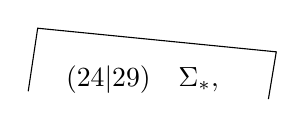
\begin{tikzpicture}[baseline]
 \node at (1.45,0) {\((\unsure{24|29})\quad\Sigma_*,\)};
 \draw (0,-0.15) -- (0.12,0.65) -- (3.15,0.35) -- (3.05,-0.25);
\end{tikzpicture}}
muni d'une relation d'ordre
\[
 \Sigma_{**}\subset\Sigma_*\times\Sigma_*
\]
ayant un graphe fermé, et tel que
\[
 \Sigma_{**}\xrightarrow{\operatorname{pr}_2=\mathrm{but}}\Sigma_*
\]
soit une \deleted{plongement}\inserted{immersion} --- plus

\margin{\textcircled{10}}
\margin{42}
